\section{Implementation Details}

As part of this work four different pieces of software were developed. We briefly describe them in the following list and delve deeper in the following subsections.

\begin{itemize}
    \item \textbf{GraphNets library}. The GraphNets library is a Python implementation of the graph network framework proposed by \cite{deepmind:graphnets}. It was developed in such a way that other people can use it in their projects too. Therefore, we have put special focus on its documentation in Section \ref{sec:gnlib}.
    \item \textbf{RankPredictor}. The RankPredictor code is a collection of Python scripts and classes which are the actual implementation of our method. The code heavily relies on the GraphNets library and implements many of its abstract classes. The code contains our models and can be used to reproduce our results.
    \item \textbf{Human evaluation tool}. The human evaluation tool is a lightweight Node.js server with a simplistic frontend that was used to determine the human performance on the pagerank task. It shows pairs of webpages and asks the user to rank them. The answers are being stored so the human accuracy on pairwise pagerank estimation can be output.
    \item \textbf{Datacrawler}. The Datacrawler served the purpose of created the dataset. In order to do so, it visits webpages, takes screenshots, collects meta information, and stores the collected data. It was developed in C++ with special focus on scalability and modularity.
\end{itemize}

The two machine learning parts (GraphNets library and RankPredictor) are both relying on the deep learning platform \textit{PyTorch}. It was preferred over the alternative \textit{TensorFlow} (\cite{abadi2016:tensorflow}) for several reasons: PyTorch supports automatic differentiation, see \cite{paszke2017automatic:pytorch}, which simplifies model analysis and debugging\footnote{With TensorFlow v2 the eager execution comes to that framework as well. By the time of writing, however, v2 was still in beta.}. Secondly, we perceive PyTorch's input pipelines as cleaner because they are more opinionated. There is only a singly primary way of defining a dataset and pre-processing pipeline. Lastly, PyTorch encourages object-oriented programming by defining the classes \texttt{torch.utils.data.Datatset} and \texttt{torch.nn.Module} from which the framework user inherits.

\subsection{GraphNets Library}
\label{sec:gnlib}

Our GraphNets library is an implementation of the graph network (GN) framework introduced by \cite{deepmind:graphnets}. It can be used to implement and train GNs in combination with the deep learning platform PyTorch. Its primary use-case is research in the field of GNs. We have developed it within the scope of this work. The framework is, however, not influenced by the pagerank aspects. It is generic and could, as-is, be used for any problem that requires GNs.

The researchers at DeepMind have implemented their own framework and have open-sourced it\footnote{GitHub repository deepmind/graph\_nets: \url{https://github.com/deepmind/graph_nets}} in late 2018. Opposed to our solution it is based on the deep learning framework TensorFlow. We chose not to use it because the development of a custom solution gave us more flexibility, a learning opportunity, and the free framework choice (PyTorch vs. TensorFlow).

In the remainder of this section we explain the components of our library and link it to the mathematical formulation of Section~\ref{sec:graphnetworks}. Furthermore, we mention specific details of the implementation which seem relevant. We close by naming potential future features and improvements.

\subsubsection{Graph Data Structures}

\begin{figure}\centering
    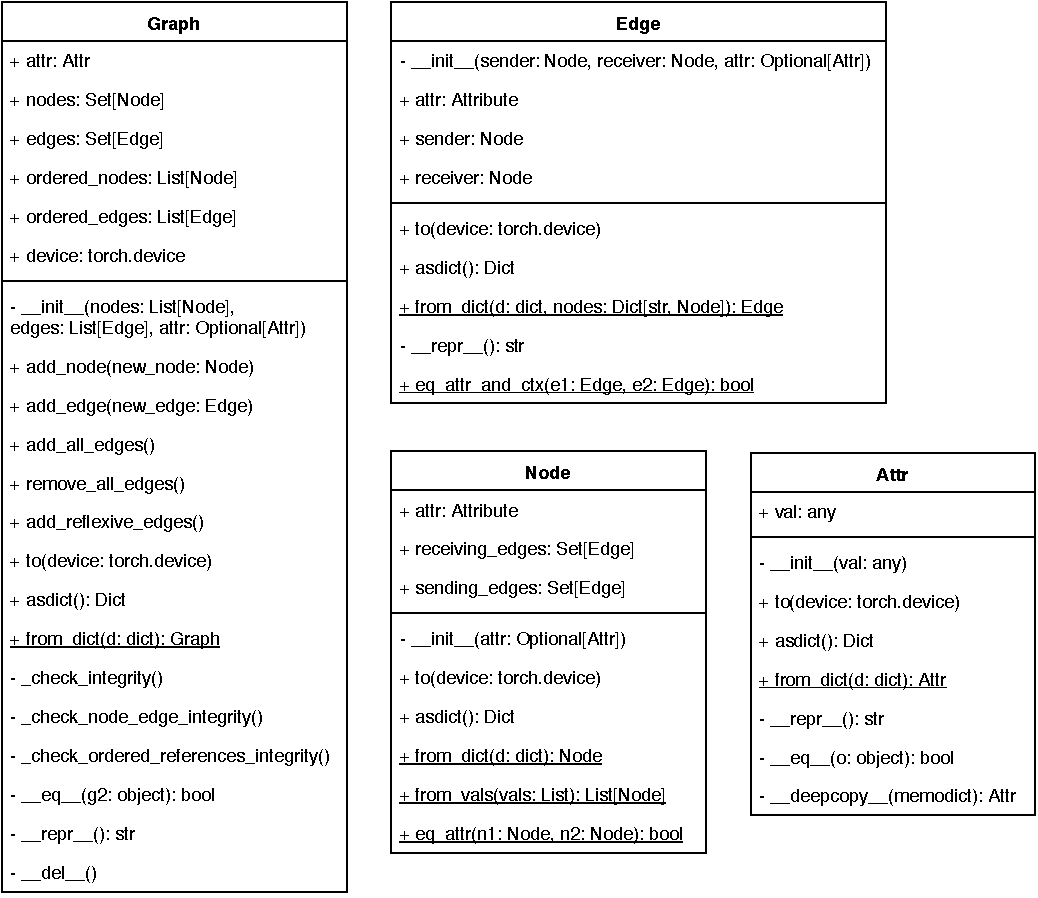
\includegraphics[scale=0.65]{resources/graphnets-datastructs}
    \caption[Class diagram of the graph network library data structure classes]{Class diagram of the graph network library data structure classes, representing a directed, attributed multigraph}\label{fig:classdiagramgndatastructs}
\end{figure}

The graph data structures are four classes, namely \texttt{Graph}, \texttt{Edge}, \texttt{Node}, and \texttt{Attribute}. They are the implementation of a directed, attributed multigraph\footnote{A multigraph is a graph which may have multiple edges (also called parallel edges). For example, there may be two edges pointing from a given node $v_1$ another node $v_2$.} with a global attribute. Here we follow the mathematical specification of \cite{deepmind:graphnets} closely. Figure~\ref{fig:classdiagramgndatastructs} depicts the classes with attributes and methods.

The \texttt{Graph} class stores references to all contained nodes and edges. They are stored in a set and in a list for performance reasons: The set allows to determine in $\mathcal{O}(1)$ time whether a node/edge is contained in the graph. The list in turn allows for $\mathcal{O}(n)$ comparison of two isomorphic graphs. The method \texttt{\_check\_integrity()} validates, whether the edges are exclusively connecting nodes contained in the \texttt{nodes} set. It also ensure that the elements contained in \texttt{nodes} and \texttt{ordered\_nodes} are equivalent (and for edges respectively). The \texttt{Graph}'s \texttt{\_\_del\_\_} method is overwritten because it traverses the graph and searches for PyTorch tensors which are placed on the GPU. Upon deletion it moves them to the CPU to ensure their garbage collection after destruction of the \texttt{Graph} object.

An \texttt{Edge} requires two nodes (sender and receiver) to be passed to its constructor. The edge adds itself to the \texttt{receiving\_edges} set of the receiver and \texttt{sending\_edges} set of the sender. \texttt{Edge} objects must therefore be created after \texttt{Node}s.

All three, \texttt{Graph}, \texttt{Node}, and \texttt{Edge} have in common that they have an attribute \texttt{attr} of type \texttt{Attr}. An attribute can hold any value in its \texttt{val} attribute. In the pagerank example, the \texttt{val} of an attribute may for instance be a tuple of screenshots.

\subsubsection{Aggregation and Update Functions}

Aggregation functions serve the purpose of converting a set of attributes into a single attribute. Update functions exist for nodes, edges, and the global state and map their attributes to new, updated attributes. In the graph network framework aggregation functions are denoted by $\rho$ and update functions by $\phi$. All aggregation functions and their relationships can be seen in the class diagram in Figure~\ref{fig:classdiagramgnfunctionsaggr}.

\begin{figure}\centering
    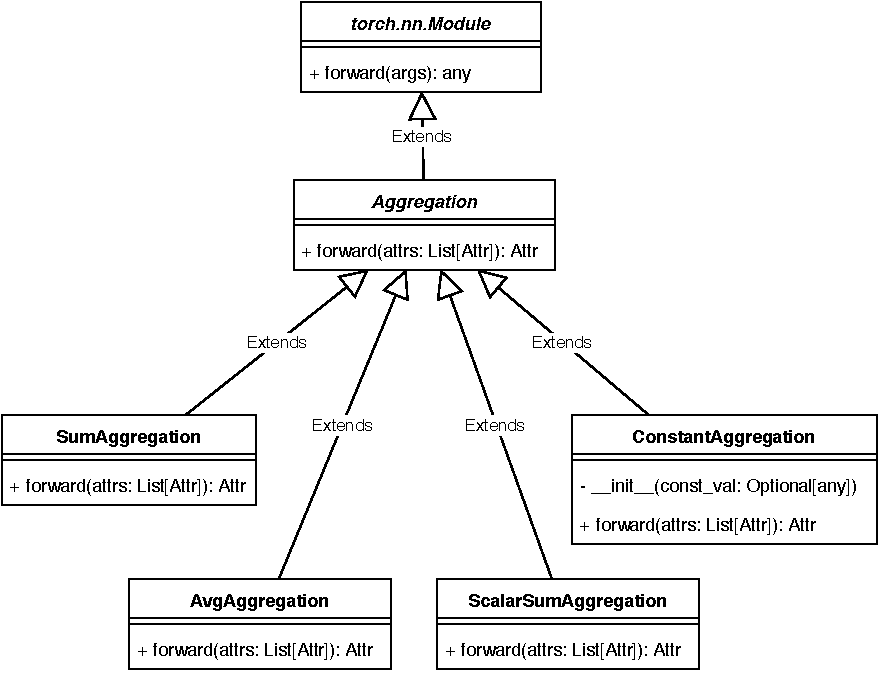
\includegraphics[scale=0.65]{resources/graphnets-functions-aggr}
    \caption{Class diagram of the graph network library aggregation functions}\label{fig:classdiagramgnfunctionsaggr}
\end{figure}

The \texttt{Aggregation} class is abstract and may be implemented by the user of our library. An aggregation can be used for nodes and edges alike. Several common, default implementations are provided, namely

\begin{itemize}
    \item \texttt{SumAggregation}: Sums up the vectors (PyTorch tensor objects) in the set of attributes (parameter \texttt{attrs}) element-wise and returns the resulting vector wrapped in a new \texttt{Attr} object.
    \item \texttt{AvgAggregation}: Works like \texttt{SumAggregation} with subsequent division by the length of \texttt{attrs}.
    \item \texttt{ScalarSumAggregation}: Operates on a list of attributes which hold scalar values, e.g. Python \texttt{float} or \texttt{int} values. It sums them up and returns the resulting value wrapped in a new \texttt{Attr} object.
    \item \texttt{ConstantAggregation}: Ignores the list of attributes entirely and returns a constant value which can be passed to the constructor. This aggregation is useful in a cases where the set of nodes or edges does not contain any useful attributes yet. For instance in the encoder of a GN.
\end{itemize}

The update functions are specific to edges, nodes, and the global state. Therefore, three abstract classes exist, namely \texttt{EdgeUpdate}, \texttt{NodeUpdate}, \texttt{GlobalStateUpdate}, corresponding to $\phi^e$, $\phi^v$, and $\phi^u$, respectively. The classes are abstract because the update may be chosen by the user of the library. The relationships can be seen in the class diagram in Figure~\ref{fig:classdiagramgnfunctionsupdate}.

\begin{figure}\centering
    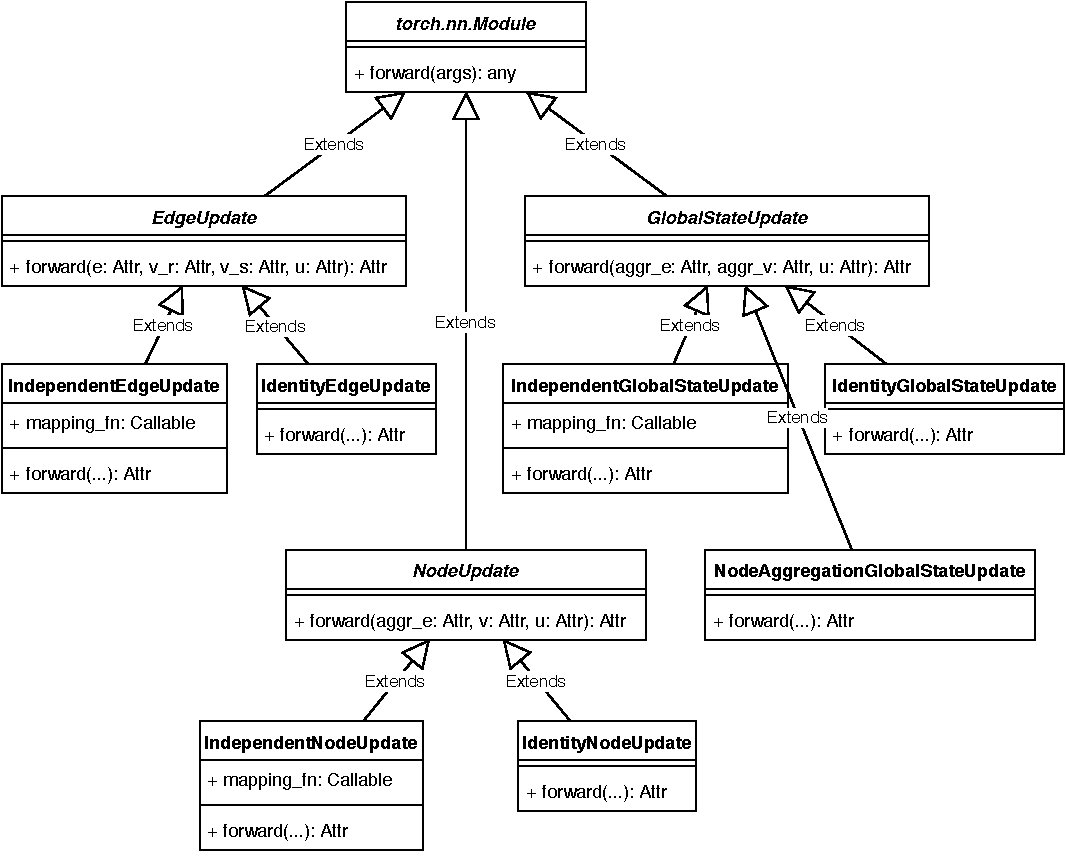
\includegraphics[scale=0.65]{resources/graphnets-functions-update}
    \caption{Class diagram of the graph network library update functions}\label{fig:classdiagramgnfunctionsupdate}
\end{figure}

For all three types of update functions, the library comes with two default implementations: First, the indepdendent update (\texttt{IndependentEdgeUpdate}, \texttt{IndependentNodeUpdate}, \texttt{IndependentGlobalStateUpdate}). An indepdentent update function takes a parameter called \texttt{mapping\_fn}. The result of a forward pass is the application of that mapping function $f_\text{map}$ to the previous edge (or node or global state) attribute. Mathematically that is \begin{align}
\phi^e\left(\bm{e}_k,\bm{v}_{r_k},\bm{v}_{s_k},\bm{u}\right)=&f_\text{map}\left(\bm{e}_k\right)\\
\phi^v\left(\bm{\overline{e}}'_i,\bm{v}_i,\bm{u}\right)=&f_\text{map}\left(\bm{v}_i\right)\\
\phi^u\left(\bm{\overline{e}}',\bm{\overline{v}},\bm{u}\right)=&f_\text{map}\left(\bm{u}\right)\,.
\end{align}Verbally described, everything but the previous attribute value is discarded and the new attribute value is computed with the mapping function.

The identity update functions leave the attribute values unaltered.

\subsubsection{GN Block}

\begin{figure}\centering
    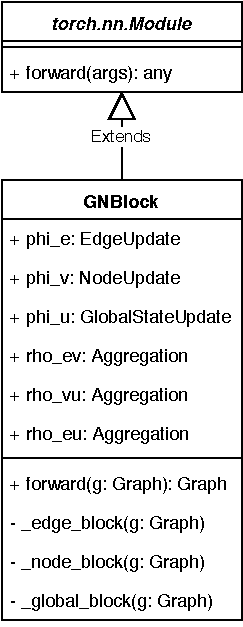
\includegraphics[scale=0.65]{resources/graphnets-block}
    \caption{Class diagram of the graph network library GNBlock class}\label{fig:classdiagramgnblock}
\end{figure}

The GN block is the core component of the library. It inherits from the PyTorch class \texttt{torch.nn.Module} (see class diagram in Figure~\ref{fig:classdiagramgnblock}). Its input is a graph and it outputs a transformed version of that graph, by passing it through the \texttt{forward} method. The implementation of \texttt{forward} is exactly matching the flow shown in Figure~\ref{fig:fullgraphblock}.

An instantiation of a \texttt{GNBlock} object requires update and aggregation functions. The correspondence between functions and attributes is shown in Table~\ref{tab:gnblockattrs}.

\begin{table}
    \centering
    \begin{tabular}{ l l l }
        \hline
        \textbf{Function} & \textbf{Attribute} & \textbf{Default}\\
        \hline
        $\phi^e$ & \texttt{phi\_e} & \texttt{IdentityEdgeUpdate} \\
        $\phi^v$ & \texttt{phi\_v} & \texttt{IdentityNodeUpdate} \\
        $\phi^u$ & \texttt{phi\_u} & \texttt{IdentityGlobalStateUpdate} \\
        $\rho^{e\rightarrow v}$ & \texttt{rho\_ev} & \texttt{ConstantAggregation} \\
        $\rho^{e\rightarrow u}$ & \texttt{rho\_eu} & \texttt{ConstantAggregation} \\
        $\rho^{v\rightarrow u}$ & \texttt{rho\_vu} & \texttt{ConstantAggregation} \\
        \hline
    \end{tabular}
    \caption[Mapping from \texttt{GNBlock} attributes to graph network functions]{Mapping from \texttt{GNBlock} attributes (see class diagram in Figure~\ref{fig:classdiagramgnblock}) to graph network functions (described in Section~\ref{sec:graphnetworks}). The default value is chosen if the attribute is left unspecified.}
    \label{tab:gnblockattrs}
\end{table}

The GN block simplifies the creation of a GN significantly. After specifying aggregation and update functions, a graph can be passed to a \texttt{GNBlock} instance is is processed by it. Listing \ref{lst:gnblock} shows this flow.

\begin{lstlisting}[
    label={lst:gnblock},
    language=Python,
    caption={Sample usage of the \texttt{GNBlock} class},
    captionpos=b
]
core_block = GNBlock(
    phi_e=CoreEdgeUpdate(drop_p),
    phi_v=CoreNodeUpdate(drop_p),
    phi_u=CoreGlobalStateUpdate(drop_p),
    rho_ev=AvgAggregation(),
    rho_vu=AvgAggregation(),
    rho_eu=AvgAggregation())

g = Graph()
# add attributed nodes and edges to g ...
g_processed = core_block(g)
\end{lstlisting}

\subsubsection{Future Features and Improvements}

The current implementation of the library is processing each graph individually. Batches can not be processed in parallel, which is due to the nature of graphs: A single batch may contain many graphs of different size and shape. A performance boost could be gained by implementing CUDA kernels for the some common update and aggregation functions that handle batches.

A useful feature would be a greater toolbox of implemented update and aggregation functions. Also, composition of GN blocks into actual networks could be simplified with pre-defined modules.

In our current implementation the critical features of the components are being unit tested. There is also an end-to-end test which trains a GN to learn the identity function, thereby ensuring PyTorch's automatic differentiation works through GN blocks. Before performing a greater refactoring (e.g. the implementation of CUDA kernels), a higher test coverage would be desirable.

\subsection{Rank Predictor}

We have dubbed our working project \textit{Rank Predictor}. It contains things such as implementation of machine learning (ML) models, dataset loader and pipeline, analysis scripts, and training orchestration scripts. Opposed to the GN code it is not a library but rather a loose collection of scripts and classes. In combination with the dataset it may be used to reproduce our results.

In this section we describe the individual components on a high level, enriched with noteworthy details.

\begin{itemize}
    \item \textbf{Analysis}: Scripts and Jupyter notebooks for post-training analysis of model weights, activations, etc.
    \item \textbf{Data}: The subfolders \texttt{data/v1} and \texttt{data/v2} contain code related to both dataset versions, respectively. For each dataset we define a class (\texttt{DatasetV1} and \texttt{DatasetV2}) which extends PyTorch's dataset class \texttt{torch.utils.data.Dataset}. The datasets only hold a list of all files in RAM and load the samples (images and the graph JSON file) on the fly, once a sample is requested. The dataset classes may be reused by researchers who want to work with our dataset as well.\\
    We split our datasets with the method \texttt{get\_threefold}. It deterministically splits the dataset on program-startup. The source code is written down in Listing \ref{lst:getthreefold}.\\
    For dataset version 2 there are two subclasses namely \texttt{DatasetV2Screenshots} and \texttt{DatasetV2Cached}. The former discards all graph information and yields lists of screenshots instead. The latter serves graphs where the nodes are attributed with cached feature vectors, previously computed by a feature extractor model.
    \item \textbf{ML models}: Our ML models are in the \texttt{model} subfolder. Each model is a class inheriting from \texttt{torch.nn.Module} with its own file. For graph networks there are commonly implementations of aggregation and update functions which we place in the model file as well.
    \item \textbf{Trainer}: Orchestration of training runs. We use TensorBoard to monitor training runs and Sacred to log experiments. Our \texttt{TraininRun} class is generic and calls an abstract \texttt{\_train\_step} method for each training step. After several steps it calls \texttt{\_run\_valid} with both train and test dataset to see how well the model performs on those dataset in evaluation mode (dropout disabled). We implement this class for graph network training, feature extractor pre-training, and training on dataset version 1. The trainer folder also contains the probabilistic ranking loss (defined in Section~\ref{sec:loss}) and accuracy metric function (defined in Section~\ref{sec:accuracy}). We have unit tested the critical functions.
\end{itemize}

\subsection{Human Evaluation Tool}
\label{sec:humanevaltool}

In order to compare the performance of our pagerank estimation model with humans, we have developed a basic evaluation tool. It allowed us to determine the accuracy of human individuals on the pagerank task.

Figure \ref{fig:humanevalscreenshot} is a screenshot of the tool. The user opens the tool in their webbrowser and sees screenshots from two webpages. Then, the user can examine both of them and must decide which one they suspect to be ranked higher. After the decision, which can be expressed either by clicking onto the page or using the hotkeys, the tool shows the next tuple. A tuple may also be skipped, for instance if one of the pages is all-black.

The pages are randomly chosen. The user can constantly see their accuracy and the number of samples they have assessed so far. Reloading the page will not result in loss, because the scores are saved in the browser's local storage. If desired, however, the score can be reset manually.

\begin{figure}\centering
    \makebox[\textwidth]{
        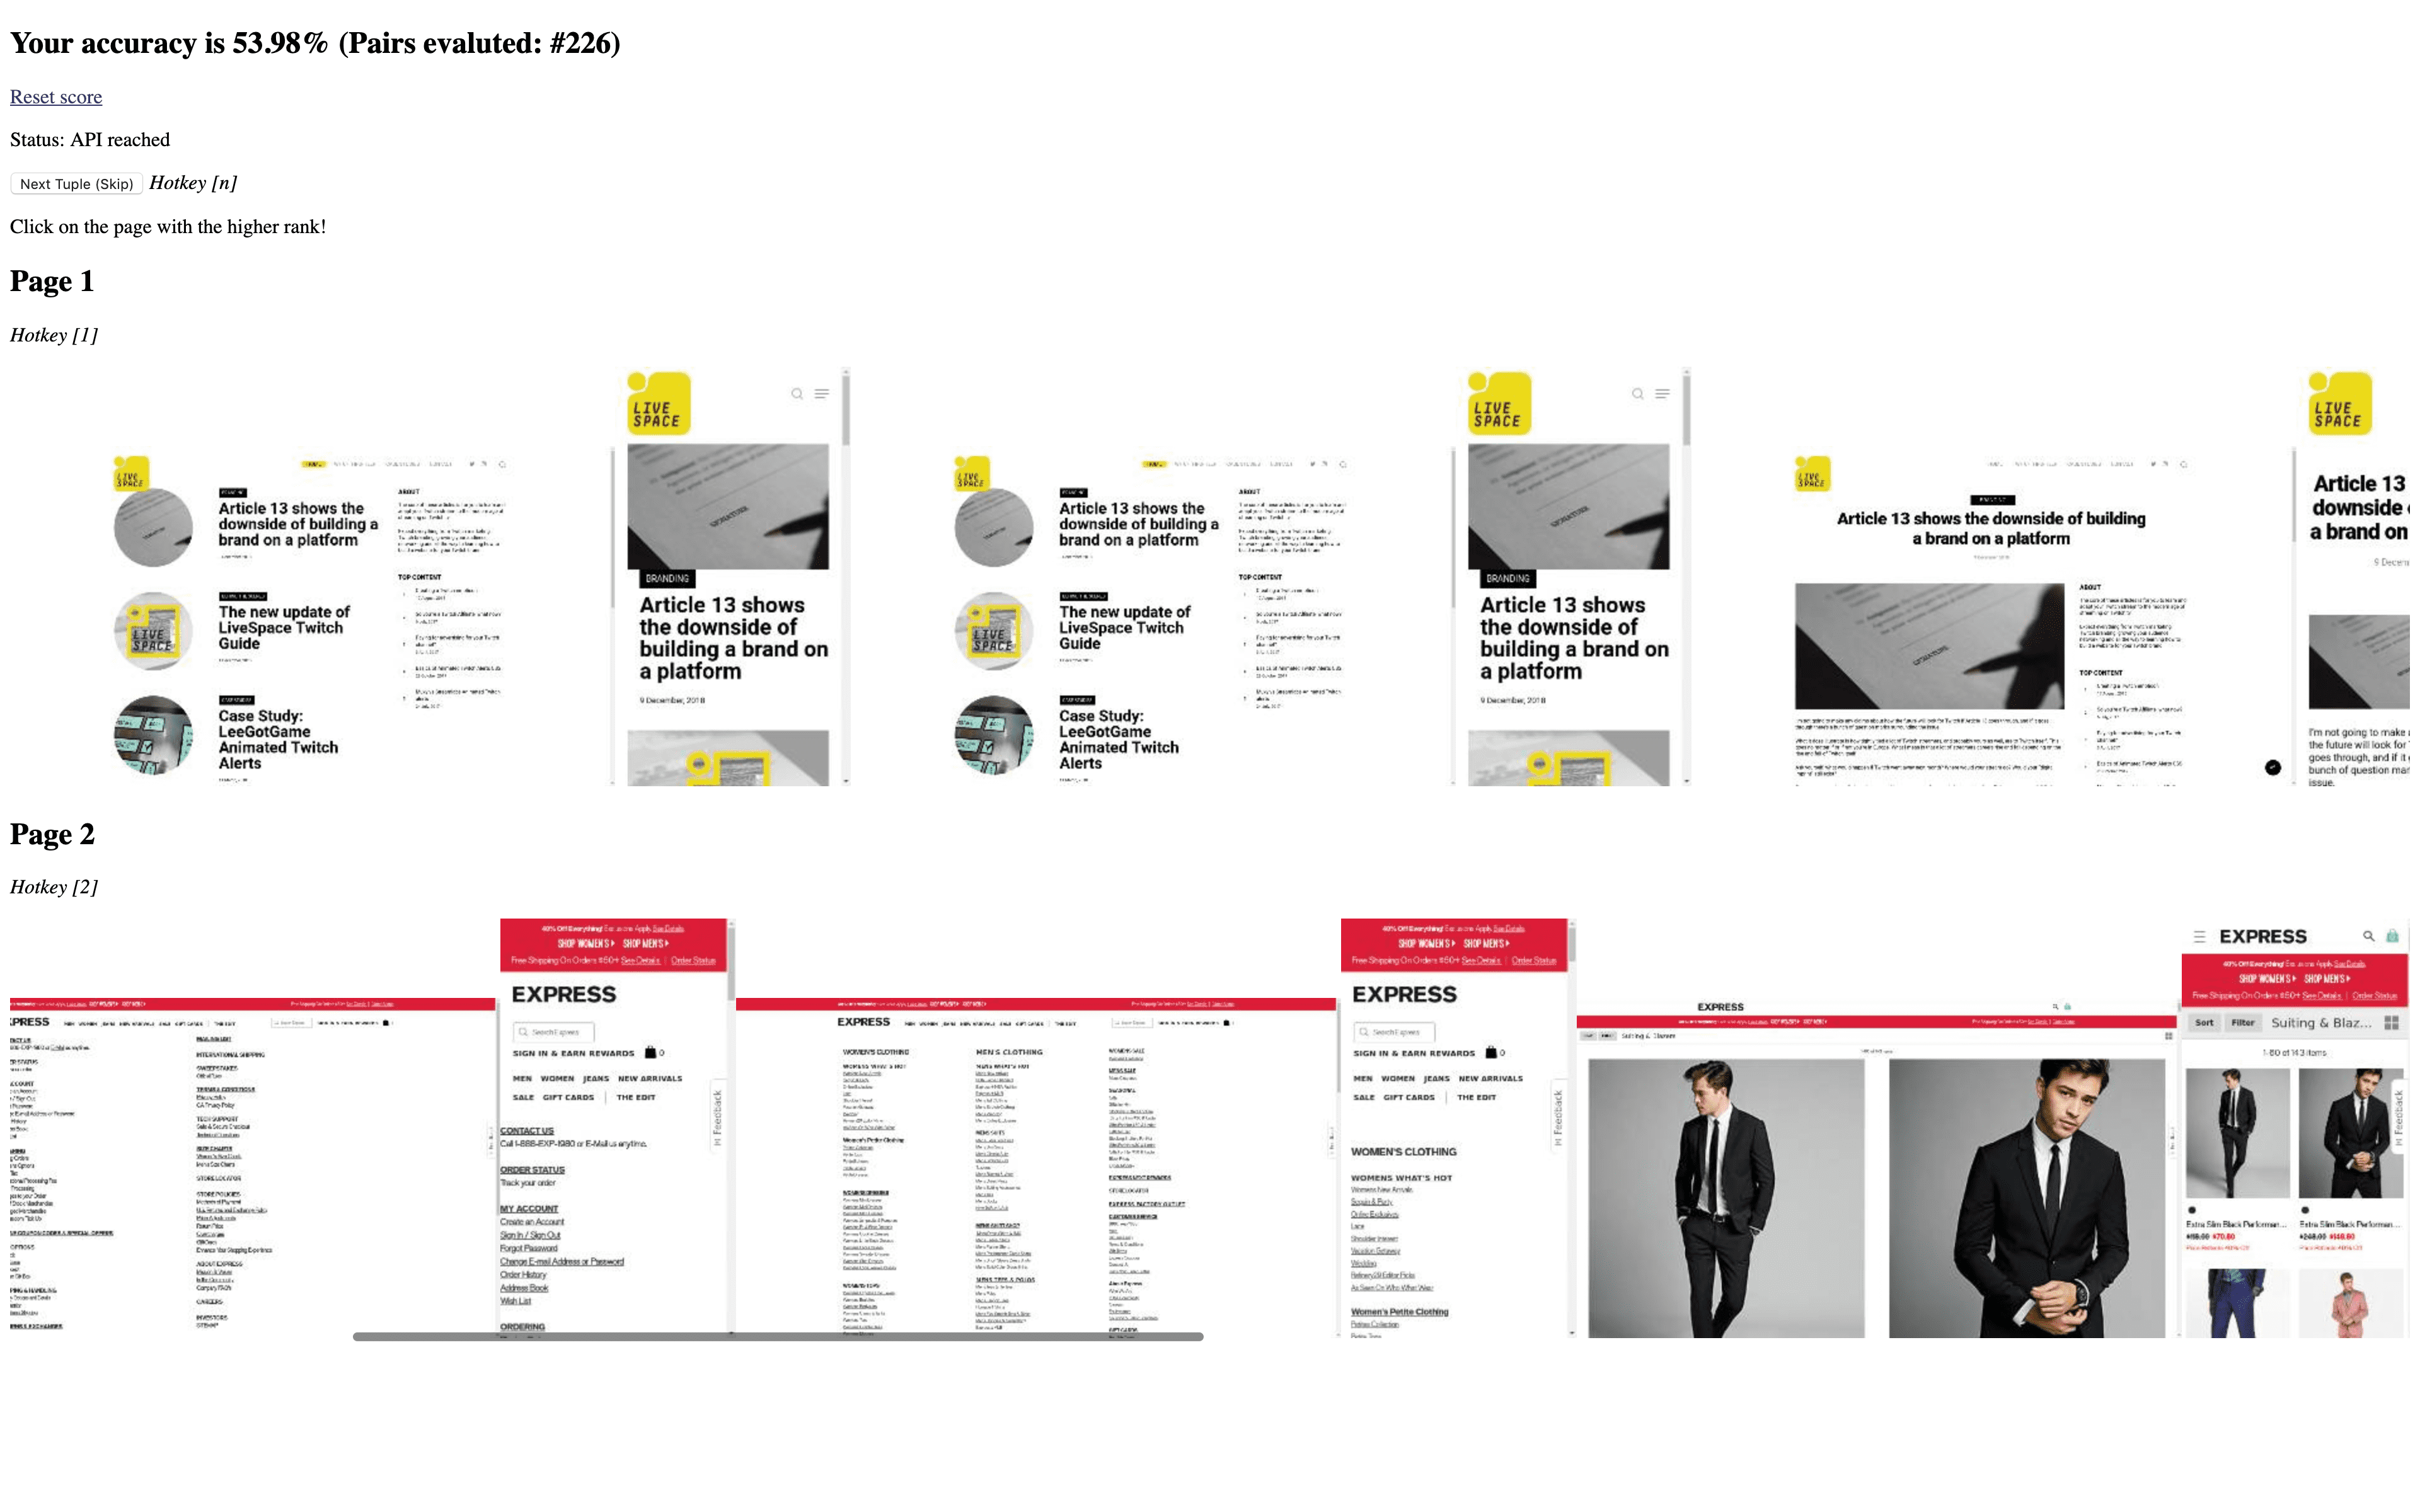
\includegraphics[width=\textwidth]{resources/human-eval-screenshot-min.png}
        }
    \caption[Screenshot of the human evaluation tool]{Screenshot of the human evaluation tool. The user has to decide which webpage they expect to have a higher rank. What would your guess be? The page on top has the rank \#68636, which is worse than \#15898, the rank of the page below. Consequently, choosing the second page is correct, here.}\label{fig:humanevalscreenshot}
\end{figure}

The tool has a Node.js backend which provides an API. It serves the dataset images, meta information such as website ranks, and random tuples. The UI is very simple and has only few CSS styling rules.

\section{Datacrawler}
\label{Datacrawler}
The datacrawler represents a very important part and has a critical role in the success of our research. The main purpose of the datacrawler is to collect data and enrich existing data. Specifically, the datacrawler is used to deliver the required dataset versions (described in Section \label{dataset} \improve{[IMPROVE] Add reference to dataset}), used to do research, develop, and train our model.

The input to the datacrawler is simply a domain, which is initially provided by the chosen ground truth in the dataset specification. The output varies between dataset versions. For example, dataset version 1 (specified in Section \label{datasetversion1}) \improve{[IMPROVE] Add reference to dataset version 1} requires a screenshot per given domain.

The following sections will describe the initial conceptual requirements for the datacrawler (\ref{datacrawler_requirements}), the decisions taken towards chosen the frameworks and programming language (\ref{datacrawler_framework_language}) and the current architecture of the datacrawler (\ref{datacrawler_architecture}). Within that the custom plugin-system with so called \textit{DataModules} are introduced (\ref{datacrawler_datamodulesystem}), all developed and consumed DataModules (\ref{datacrawler_screenshot_datamodule}, \ref{datacrawler_mobilescreenshot_datamodule} \improve{[IMPROVE] Add missing refs to new datamodules}) and their interplay as a whole unit is described (\ref{datacrawler_workflow}). \info{[INFO] You might add a section with "Calculating the Graph" or "Outputing the dataset"} In the last section we will discuss how we used state-of-the-art technologies and designed an architecture to scale the datacrawler to dramatically reduce the analysis time (\ref{datacrawler_scale}).

\subsection{Requirements}
\label{datacrawler_requirements}
In general all dataset version specifications (\ref{datasetversion1}, \ref{datasetversion2}) can be seen as requirements for the datacrawler. While a specification generally describes how the given dataset version should look, it also implicitly defines required functionality for the datacrawler. A specifications such as the demand for a screenshot of the given website, implicitly requires the datacrawler to be able to render and take a screenshot of the website.

One of the major requirements for the datacrawler was to find a convenient way of emulating a web browser. This requirement raised from the fact that the main goal of our research was to evaluate a given website and calculate a rank depending on the user experience of the user during their visit of the website. This requirement is furthermore underlined by the fact that any other approaches to calculate attributes of a domain, such as the download size or loading time, would ultimately lead to distortion of the data. Another fact is that for attributes such as screenshot the given website has to be interpreted and rendered on the screen with the highest possible compatibility. The browser was primarily designed for this purpose.

The accessibility to \textit{low-level} information of a website represents another important requirement and is raised from the emulation of a browser. This means that the datacrawler had to have the possibility to access information such as the \textit{HTTP-Request} (\ref{datacrawler_mobilescreenshot_datamodule}) or \textit{Document Object Model} (\ref{datacrawler_url_datamodule}) to be able to calculate specific attributes. So being able to read and manipulate internal data structures or even to inject own Javascript (\ref{datacrawler_screenshot_datamodule}, \ref{datacrawler_mobilescreenshot_datamodule})  represents another inevitable requirement for the datacrawler.

Another requirement was the flexibility regarding to be calculated attributes. In this case flexibility means that each attribute should be calculated independently from each other generating high flexibility in choosing which attributes should be calculated. This flexibility raised from the iterative process of dataset specification: It might happen that dataset version $i$ requires some certain attributes whereas dataset version $i+1$ does not. This flexibility was required and led to a sophisticated architecture such as the \textit{DataModule-System} (\ref{datacrawler_datamodulesystem}), which makes it possible to directly feed the dataset specification into the datacrawler.

Lastly scalability and efficiency in terms of time represented two major requirements for the datacrawler. Considering the huge amount of domains to be analysed, the datacrawler had to be horizontally scalable to allow the analysis of multiple domains at once, and efficient in terms analysis time and start-up time. An inefficient and not scalable datacrawler would lead to multiple days of required analysis time and high infrastructure costs.

\subsection{Chromium Embedded Framework}
\label{datacrawler_framework_language}

\subsection{Datacrawler Architecture}
\label{datacrawler_architecture}

\subsubsection{DataModule-System}
\label{datacrawler_datamodulesystem}

\subsubsection{Screenshot-Datamodule}
\label{datacrawler_screenshot_datamodule}

\subsubsection{MobileScreenshot-Datamodule}
\label{datacrawler_mobilescreenshot_datamodule}

\subsubsection{URL-Datamodule}
\label{datacrawler_url_datamodule}

\improve{[IMPROVE] Add documentation for new datamodules}

\subsubsection{Datacrawler Workflow}
\label{datacrawler_workflow}

\subsection{Scaling the Datacrawler}
\label{datacrawler_scale}

\subsubsection{Requirements}
\label{datacrawler_scale_requirements}

\subsubsection{The Scale Architecture}
\label{datacrawler_scale_architecture}



